\section{污染物排放}
\subsection{概述}
\subsection{污染物的危害}
\begin{enumerate}
    \item 改变大气和降水的特性;
    \item 对植被有害;
    \item 污染和破坏了各种材料;
    \item 可能提高人类的发病率和死亡率。
\end{enumerate}

\subsection{排放的量化描述}
\subsubsection{排放因子}
\begin{equation}
    \mathrm{EI}_i = \frac{m_{i,\mathrm{emitted}}}{m_{\mathrm{F,burned}}}
\end{equation}
对于碳氢化合物在空气中的燃烧,排放因子可以由指定测量的组分浓度(摩尔分数)和所有含碳组分的浓度来决定。
\begin{equation}
    \mathrm{EI}_i = \left(\frac{\chi_i}{\chi_\mathrm{CO} + \chi_\mathrm{CO_2}}\right)\left(\frac{x MW_i}{MW_\mathrm{F}}\right)
\end{equation}

排放因子的测量与任何(比如)空气稀释效果无关。

\subsubsection{折算浓度}
实际应用中,通常将排放浓度折算为燃烧产物中特定含氧量下的值。目的在于排除各种稀释情况的影响,从而能够对污染物排放进行客观的比较。

\subsubsection{各种特定的排放测量}
比质量排放=污染物的质量流量/制动力。

\subsection{预混燃烧过程的排放}

\subsubsection{氮氧化物}

\begin{enumerate}
    \item 当量比为1的层流预混燃烧火焰中,压力的影响大: 低压下NO的形成由快速NO机理中的费尼莫尔(HC-N2)以及O和OH超平衡路径来控制。高压条件下(如10atm)热力型机理产生了一半以上。
    \item 富燃料层流预混火焰,当量比的影响大。随着混合物中燃料逐渐增多,快速NO机理起主导作用,当量比为1.32时形成了约95\%NO。(总的NOx也少)。
    \item 全混流反应器(完全混合的反应器)。在反应物和产物发生强烈的返混时,快速NO机理中的超平衡O和OH的反应路径控制贫燃混合物的反应;快速NO机理中的Fenimore控制化学当量下以及富燃混合物的燃烧。
\end{enumerate}

控制策略:对于热力型NO,需要很高的活化温度。
\begin{itemize}
    \item 降低峰值温度:将废气(烟气)与新鲜空气或燃料混合。废气(烟气)再循环的作用:在给定热释放量的条件下,增加燃气的比热容,降低燃烧温度。
    \item 推迟火花点火时间:较晚的点火时间可改变燃烧过程,使最高压力刚好出现在发动机的上止点, 从而降低压力和温度。但是这样会牺牲燃油经济性。
    \item 分级燃烧:当然实际不是这样的。
    \begin{enumerate}
        \item 利用富燃燃烧的高稳定性和低NOx特性完成初步过程
        \item 在贫焰燃烧阶段将产生的CO和H2完全燃烧完
    \end{enumerate}
    \item 催化后处理技术。
\end{itemize}

\subsubsection{一氧化碳}
生成机理:
\begin{enumerate}
    \item 特定的燃烧温度下CO\(_2\)的离解;
    \item 冷壁面熄火;
    \item 未燃尽燃料部分氧化过程。
\end{enumerate}

\subsubsection{未燃烃}
\begin{enumerate}
    \item 壁面熄火产生的碳氢化合物绝大多数最终都会与高温气体混合并被氧化掉,但是在缝隙的入口和里面都会产生未燃碳氢化合物,例如在活塞端环槽脊上、环形密封处、螺旋火花塞的缝隙中;
    \item 壁面上油层对燃料的吸附和解吸附;
    \item 气缸内火焰的不完全传播;
    \item 燃料高温热解及部分氧化。
\end{enumerate}

\subsubsection{催化后处理技术}
\begin{figure}[H]
    \centering
    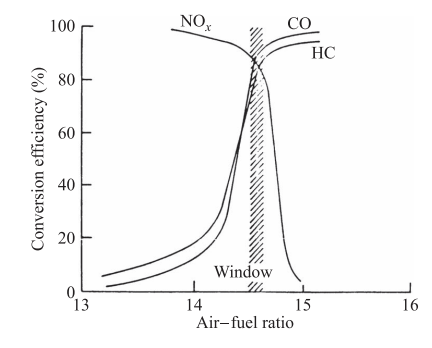
\includegraphics[width=.3\textwidth]{img/three-way.png}
\end{figure}

实际情况是不太好控制的。

\subsubsection{颗粒物}
预混燃烧,各种燃料形成碳烟的趋势不仅与燃料结构有关,还与火焰温度有关。

\subsection{非预混燃烧的排放}


\subsubsection{氮氧化物}
氮氧化物-工业燃烧设备控制策略
\begin{itemize}
    \item 低过量空气:只能有限的降低NOx排放,因为过量空气减少使CO排放增加;
    \item 分级燃烧:上游燃烧器在富燃料状态下运行,下游燃烧器只提供空气;这项技术可使NOx的减排达到10\%~40\%;
    \item 降温:在燃气工业锅炉中,用烟气再循环后, NOx的减排效果可达50\%~85\%。也可以向燃烧器中喷水来降低火焰温度。
    \item 低Nox燃烧器:还是分级燃烧的原理。
    \item 富氧燃料燃烧:加入足够大量的氧气,使氮气浓度的降低超过了燃烧温度增加的影响。
    \item 再燃:燃料总量的15\%将被直接送往贫燃区域的下游进行再燃。在再燃区内(当量比>1),NO将会和碳氢化合物及中间物质(如HCN)反应而使其降低。最后加入额外的空气,保证再燃燃料最终能燃烧完全。运用再燃技术的锅炉一般都能将NOx的排放量减小60\%。
    \item 选择性非催化还原(SNCR)-“喷氨法”。
    \item 选择性催化还原(SCR)。NOx的减排可以更大,而且操作温度更低。但是几乎是多有脱硝技术中最昂贵的,因为初期投资和运行过程中催化剂的更换成本都很高。
\end{itemize}

\subsubsection{未燃烧和一氧化碳}
\textbf{未燃碳氢化合物和CO}:

\textbf{主要途径}
\begin{enumerate}
    \item 存在过度贫燃区域难以支持快速的燃烧反应。火焰不会在过度贫燃区域内传播,在这个区域燃料发生高温热解形成部分氧化的产物,如醛类和CO。
    \item 火焰中形成过度富燃料的区域,而且没有额外的空气补充进来,或者没有足够的时间使氧化反应进行完全。
\end{enumerate}
其他途径包括:壁面熄火(柴油机)、由二次风或稀释空气的射入引起的熄火(燃气轮机)、喷管段残留燃料的滴入(柴油机)、未充分雾化的燃料液滴(燃气轮机,偶然发生)。

\textbf{颗粒物}:
燃煤产生的矿物质飞灰可以通过静电除尘等手段从尾部烟气中去除。非预混燃烧产生的主要颗粒物是碳烟。碳烟在扩散火焰的富燃区域内进行,形成的碳烟是否会从火焰中放出取决于碳烟的生成和氧化过程的平衡关系。设计燃烧系统时,使碳烟在形成前先被氧化和增加氧化速度都可以降低碳烟的排放。柴油机,燃烧后进行颗粒捕集。

\textbf{硫化物SOx}

SOx的产生:在燃烧过程中,燃料中的硫都以SO2或SO3的形式被排出,统称为SOx。控制SOx的途径:去除燃料中的硫,或去除烟气中的SOx。